%!TEX program = pdflatex

\documentclass[a4paper, 12pt]{article}

\usepackage{geometry}
\geometry{a4paper,
total={170mm,257mm},left=2cm,right=2cm,
top=1cm,bottom=2cm}

\usepackage{mathtext}
\usepackage{amsmath}
\usepackage[T2A]{fontenc}
\usepackage[utf8]{inputenc}
\usepackage[english,russian]{babel}
\usepackage{graphicx, float}
\usepackage{tabularx, colortbl}
\usepackage{caption}
\captionsetup{labelsep=period}

\newcommand{\parag}[1]{\paragraph*{#1:}}
\DeclareSymbolFont{T2Aletters}{T2A}{cmr}{m}{it}
\newcounter{Points}
\setcounter{Points}{1}
\newcommand{\point}{\arabic{Points}. \addtocounter{Points}{1}}
\newcolumntype{C}{>{\centering\arraybackslash}X}

\begin{document}
%\maketitle

\begin{titlepage}
    \vspace*{\fill}
    
    \begin{center}
        
\includegraphics[scale=0.8]{res/MIPT.pdf}
        \\[0.7cm]\Huge Московский Физико-Технический Институт
        \\[2cm]\LARGE Отчет о выполнении лабораторной работы 
        \\[0.5cm]\noindent\rule{\textwidth}{1pt}
        \\\Huge\textbf{5.1.2 \\ Эффект Комптона}
        \\[-0.5cm]\noindent\rule{\textwidth}{1pt}
    \end{center}
    
    \vspace*{\fill}
    
    \begin{flushleft}
        Выполнили: \hspace{\fill} Группа:
        \\Костылев Владислав \hspace{\fill} Б01-206
    \end{flushleft}
\end{titlepage}

\setcounter{page}{2}


\begin{abstract}
    \textbf{Цель работы:} \\
    
    \textbf{В работе используются:} 
\end{abstract}

\tableofcontents
\newpage

\section{Теоретическая справка} 
    
    % \begin{figure}[H]
    %     \centering
    %     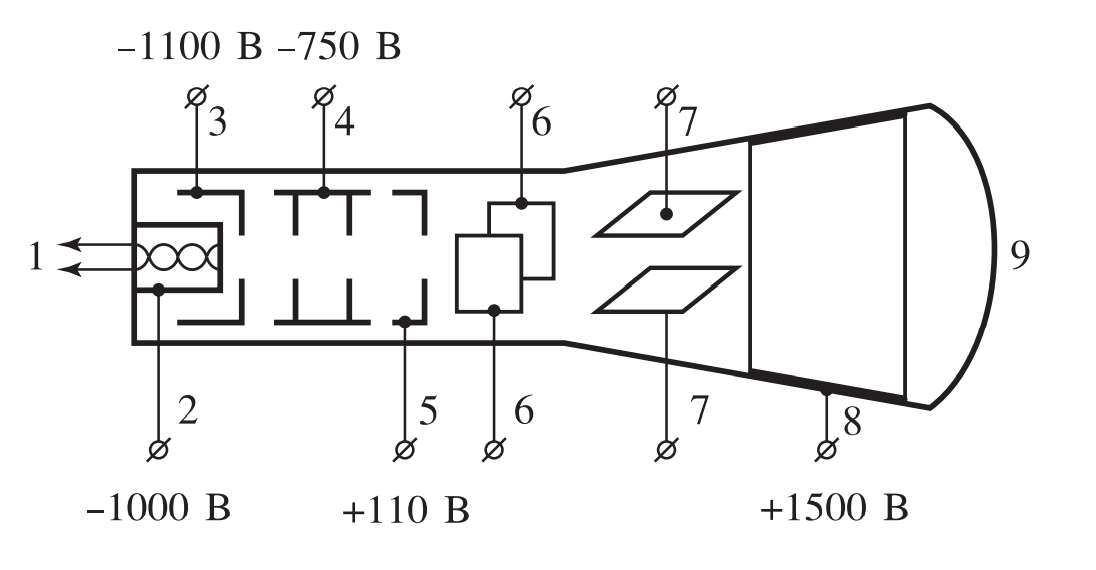
\includegraphics[width=0.7\linewidth]{1.png}
    % \end{figure}

% \section {Методика измерений}
    
    
\section{Результаты измерений и обработка данных} 

    
\section{Заключение}
    
    
\end{document}
